\documentclass[12pt]{article}
\usepackage{amsmath,amsfonts,fullpage,amsthm,graphicx}

\newtheorem*{theorem}{Theorem}
\newtheorem*{fact}{Fact}
\newtheorem*{goal}{Goal}
\newtheorem*{idea}{Idea}
\newtheorem*{defn}{Definition}
\newtheorem*{ex}{Example}

%Style section
%\setlength{\textheight}{10in}
%\setlength{\textwidth}{7in}
%\hoffset=-0.75in
 \pagestyle{plain}
% \setlength{\topmargin}{0in}
% \setlength{\headsep}{0in}
% \setlength{\oddsidemargin}{0in}
% \setlength{\evensidemargin}{0in}

\begin{document}


\pagestyle{empty} %use this to get rid of page numbers

\noindent
{Math 166 \hskip 1.5 truein  Names:\ \hrulefill}

\noindent
%\vskip 0.3truein
%\bigskip
%\noindent
{Partial fun with partial fractions}

\noindent  \hskip 3.5 truein  Section Number:\ \hrulefill
\medskip

\begin{goal} \rm
Evaluate integrals by partial fractions and/or other methods
\end{goal}
%\smallskip

\begin{enumerate}
%\setcounter{enumi}{-1}
%\item (Review)
%Write an expression for each of the six trig functions in terms of the lengths of the sides of the right triangle below:

%\medskip
%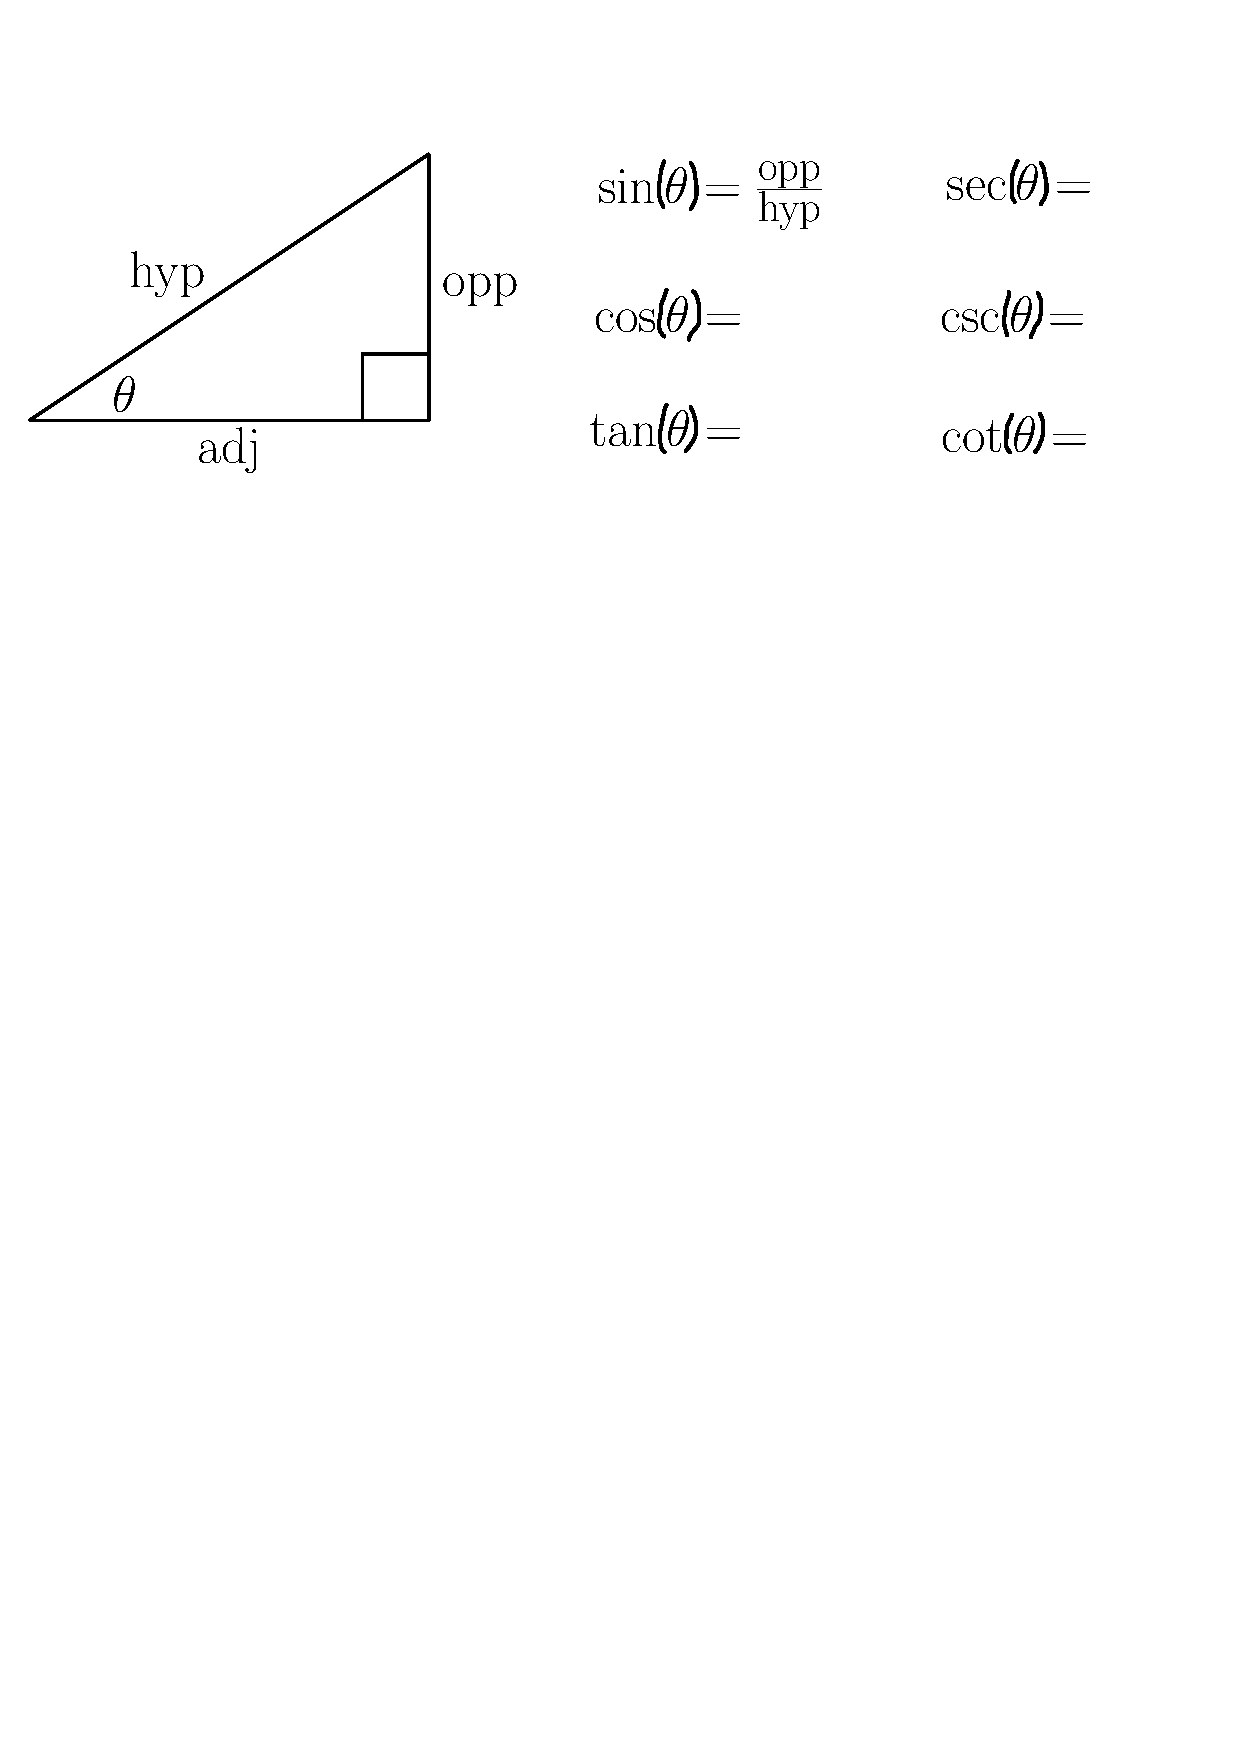
\includegraphics[scale=.5]{right_triangle.pdf} 

%\bigskip
\item Evaluate $\displaystyle\int\frac{x+8}{x^2+x-2} \  dx$ using the steps for partial fractions.
\vfill
\vfill\vfill\vfill
\item Suppose you wanted to evaluate these integrals using partial fractions. What is the form of partial fractions you would use? 
\begin{enumerate}
\item $\displaystyle\int  \displaystyle\frac{x}{(2x-1)^{4}} \ dx$

\vfill

\item $\displaystyle\int  \displaystyle\frac{22x+4}{(x-3)^2(x^2+1)} \ dx$
\vfill
\end{enumerate}





%\item Evaluate $\displaystyle\int\frac{x^2+2x-1}{2x^3+3x^2-2x} \  dx$ using the steps for partial fractions.

\vspace{2.75in}
%\item Evaluate $\displaystyle\int\frac{7x-4}{(x+2)(x-1)^2} \  dx$ using the steps for partial fractions.

\vspace{2.75in}
\item Evaluate  $\displaystyle\int  \displaystyle\frac{(5x^3+1)(x^2+x)}{(x^3-x)(x-1)} \ dx$. First, be sure to factor the denominator fully and do any algebraic simplification. 


\vspace{2.75in}
\item Evaluate integral 2(a) by a method other than partial fractions. What method did you use?

\newpage

\item Compute the following integral 
\[
\int \frac{dx}{x^2 + 6x + 8}
\]
\vfill

%\vspace{2in}
\item Use partial fractions to write integral 2(b) as the sum of several simpler integrals. Decide which of those integrals you can integrate. Integrate the ones you can, and explain why the methods you currently know fail to integrate the others.
\vfill
\vfill




\end{enumerate} 

\end{document}
